% Progress report for CS565
 
\documentclass[a4paper,12pt]{article}
\usepackage{algorithm, algorithmic}
\usepackage{graphicx}

\title{Fast Volume Visualization with Ray Casting}

\author{Eray \"Ozkural}
\date{\today}
\begin{document}

\maketitle

\newpage

\section{Introduction}

\subsection{The Need for Volume Visualisation}

Three dimensional data has been employed in many fields. In medicine
it is used to represent the information coming from a magnetic
resonance (MR) or a computed tomography(CT) machine. Geologists use
three dimensional data for many purposes varying from seismic
explorations to locating petrol oil reservoirs. In Confocal Microscopy
the detailed structures of biological specimens are stored in three
dimensional arrays. In engineering, dynamics of the fluids in designed
systems are explored with three dimensional data showing how the fluid
behaves.
 
But bare three dimensional array of data, especially with an immense
size, is hard to understand for human beings.  We need to visualize
the three dimensional information in order to grasp it, but the
quantity of data in the fields of study mentioned above often exceeds
our imagination.

At this point, volume visualisation establishes itself as a valuable
tool for us. The volume visualizer projects a view of the three
dimensional dataset onto a two dimensional image plane, aiding us in
comprehension of the structure within the data. The figure ~\ref{smb}
represents a three dimensional medical data by making use of the
volume visualisation technique.

\begin{figure}  
\begin{center}  
  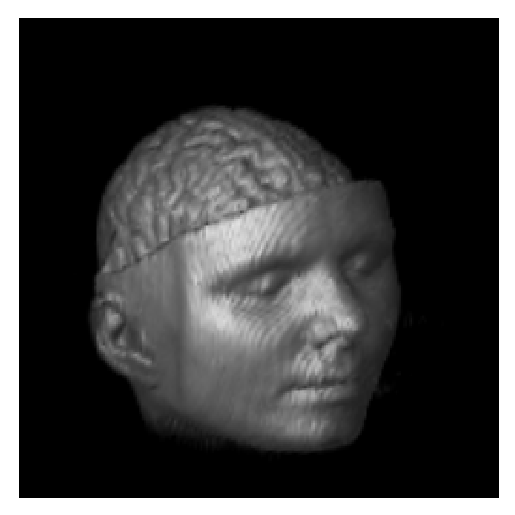
\includegraphics{brainsmall1.eps}
\caption{A simple grey scale image generated by volpack-1.0 library}
\label{smb}
\end{center}
\end{figure}

 

%\subsection{Volume Visualisation Methods}
%
% Volume Visualisation methods are divided into two: direct volume rendering 
%(DVR) and surface-fitting (SF).
%
% Direct volume rendering pictures a two dimensional image without using any
%geometrical primitive from the three dimensional array. Since DVR must be 
%traverse entire dataset not as fast as SF. But although DVR is slower 
%then the SF, it can be used to display a cut in the volume easily and 
%can cope with the amorphous  phenomenon such as clouds, fluids, and gases.
%  
% Different from DVR SF     

\subsection{Volume Rendering}

Volume rendering is the computer implementation which simulates the physical
the behavior of light, propagating in a colored semi-transparent gel.

A volume renderer takes a three dimensional array of samples, assigns
opacity and color values to each member of the three dimensional array
and then projects them on a image plane, by blending their colors
according to their transparencies.

The array, which it takes as input is called \emph{volume} and each
sample on a cell of the three dimensional matrix is called a
\emph{voxel}. A voxel of a data set can either represent a small cube
in space or a sample point of a continuous function, which we are going to use
for our volume visualisation algorithm.

In real life the interaction of light with a three dimensional
semi-transparent gel is too complicated. It involves many
possibilities for a light ray such as being absorbed, scattered or
emitted by the volume.  Furthermore, there is in physical world the
cases of fluorescence or phosphorescence reaction. But these
complexities are superfluous for volume rendering.

\subsubsection{Volume Rendering Equation}

For Volume Rendering the physical phenomenon can be approximated to
finding the color value of each pixel $x$ on two dimensional image
plane by adding color contributions of all voxels on the viewing
ray intersecting with the image plane in that particular pixel $x$ as
it is shown in figure \ref{svv}.

\begin{figure}[ht!]     
\begin{center}  
  \includegraphics{simplevolumevis.eps}
\caption{The value of pixel $x$ is computed by summing color contributions
  of voxels standing between $x$ and $x_{b}$.}
\label{svv}
\end{center}
\end{figure}

The color value $L(x)$ for the vertex $x$ on image plane can be found
with the simplified function \ref{eq:vr}. In this function, we
assume that the number of voxels on the viewing ray is $n$ and each
voxel has the color value $c_{i}$ and opacity value $\alpha_{i}$. The
opacity value $0$ corresponds to full transparency and $1$ corresponds
to total opacity.

\begin{equation} 
\label{eq:vr} 
L(x) = \sum_{i=0}^{n-1} c_{i} \prod_{j=0}^{i-1} 1-\alpha_{i}
\end{equation}
 
The volume rendering function ~\ref{eq:vr} , which calculates the
color value for a pixel on the image plane, is called the
\emph{volumetric composing equation}. It adds the color values by
multiplying them with the approximated energy they receive. The
approximation for energy value is done by multiplying the opacities
through the first voxel to the current voxel.

\subsubsection{Data Representation}

As it is mentioned above, a sample in a three dimensional matrix can
be interpreted either as a box in space or a sample point of a
continuous function.

If the latter is assumed, as we will do for our implementation,
in equation \ref{eq:vr} the attributes of the
mentioned voxels do not have to come directly from the three
dimensional array since the values on that array would be just sample
values of a continuous function at arbitrary coordinates.

These arbitrary coordinates correspond to a grid in real life.  As it
is also shown in figure \ref{grid}, the grid, to which the real
life coordinates belong, may be in three types; either unstructured,
curvilinear or regular. Regular sampling grids take samples from the
real world so that each sample has a uniform distance to other
samples. A curvilinear grid is warped form of a regular grid so that
the edges are are no further linear. An unstructured sampling grid
takes its samples from the real world arbitrarily.

Through the whole work we are going to work with regular sampling
grids, since they are common and fast because of their simplicity.
While using regular grids,  the required values of the continuous function
are interpolated by using some function on the three
dimensional array. This process is called \emph{Reconstruction} or
\emph{Resampling}.


\begin{figure}  
\begin{center}  
  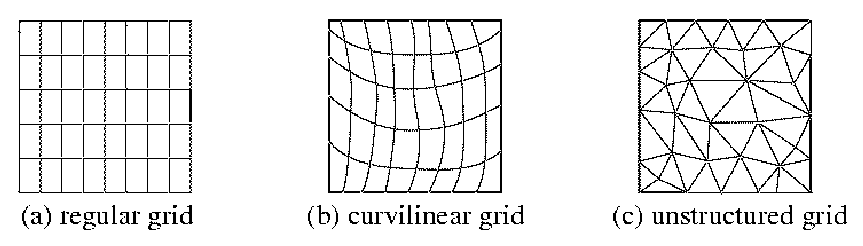
\includegraphics{grids.eps}
\caption{ Examples of sampling grids.}
\label{grid}
\end{center}
\end{figure} 
    
\subsubsection{Visualisation Process}

As mentioned in the preceding text, the three dimensional array
contains only sample values. Thus, the values $c_{i}$ and $\alpha_{i}$
used in function \ref{eq:vr} should be computed from these sample
values by two functions.

The function which maps samples to an $\alpha_{i}$ for an arbitrary point
in volume is called
\emph{classification function}. In our work classification functions
are omitted. We assume that classification is done prior to rendering.

The other function which maps sample values into a color value for
a point is called \emph{shading function}. Differing from the classification
function, shading function depends on other variables such
as viewing direction and light source direction. In our implementation, shade
function will be composed of a standard Phong shader and
arbitrary functions to implement different illuminations.

Beside the two topics another important factor effecting the
visualisation is view point and projection type. We will use parallel
projection due to its simplicity so that it will facilitate a reasonable
sample implementation.

Due to the complexity of the operations at this point, we don't
consider a fully interactive rendering system.
% The user will be able
% to select the viewport specifications, and a number of other options
% with the GUI an according to the shading function and classification
% function the desired picture will be generated.
    
\section{Background}
  
\subsection{Volume Rendering Algorithms}  

There are actually four classes of volume rendering algorithms:ray
casting, splatting, cell projection and multi-pass resampling. For our
purposes, we shall be examining ray casting and splatting
algorithms. The hybrid system will be mentioned in next sections.

Cell projection is used with non-regular grids. Since we are going to
work with regular grids cell projection algorithms remain out of our
focus.  Multi-pass algorithms are conceived for parallel systems.
At this stage we are going to implement only serial programs, so
this type of algorithms is not related to us.

\subsubsection{Ray Casting} 

Ray Casters are image order algorithms. They traverse the volume from
image space to object space. This means the image
space iterations stand in outer loops as it is in algorithm
\ref{alg:rc}.

\begin{algorithm}
\caption{Ray Casting}
\label{alg:rc}
\begin{algorithmic}
  \FOR{ $y_i \gets 1$ to ImageHeight} \FOR{ $x_i \gets 1$ to
    ImageWidth} \FOR{ $z_i \gets 1$ to RayLength} \FORALL{ $x_o$ in
    $ResamplingFilter(x_i,y_i,z_i)$ } \FORALL{ $y_o$ in
    $ResamplingFilter(x_i,y_i,z_i)$ } \FORALL{ $z_o$ in
    $ResamplingFilter(x_i,y_i,z_i)$ }
  
  \STATE $ContributeVoxel(Voxel[x_o,y_o,z_o],ImagePixel[x_i,y_i])$
  \ENDFOR \ENDFOR \ENDFOR \ENDFOR \ENDFOR \ENDFOR
\end{algorithmic}
\end{algorithm}

The disadvantage of these algorithms is that they do not access the
volume in storage order and they require costly addressing
arithmetic.

\subsubsection{Splatting}

Contrasted to ray casting these types of algorithms operate in object
order. They project the volume onto the image plane, meaning that they
iterate over object coordinates in the outer loops as in algorithm
\ref{alg:spl}.

\begin{algorithm}
\caption{Splatting}
\label{alg:spl}
\begin{algorithmic}
  \FOR{ $z_o \gets 1$ to VolumeDepth} \FOR{ $y_o \gets 1$ to
    VolumeHeight} \FOR{ $x_o \gets 1$ to VolumeWidth} \FORALL{ $z_i$
    in $ResamplingFilter(x_o,y_o,z_o)$ } \FORALL{ $y_i$ in
    $ResamplingFilter(x_o,y_o,z_o)$ } \FORALL{ $x_i$ in
    $ResamplingFilter(x_o,y_o,z_o)$ } \STATE
  $ContributeVoxel(Voxel[x_o,y_o,z_o],ImagePixel[x_i,y_i])$ \ENDFOR
  \ENDFOR \ENDFOR \ENDFOR \ENDFOR \ENDFOR
\end{algorithmic}
\end{algorithm}

The major drawback in Splatting is the expensive resampling, however
the addressing arithmetic is much simpler.

\subsection{An Efficacious Ray Casting Algorithm}

First, we will implement an efficient ray caster which makes
parallel projection. This will give us a platform on which we can
build more complicated applications, test our objects for new
applications, and serve as a sample implementation.

\begin{algorithm}
\caption{Efficient Ray Casting}
\label{alg:src}
\begin{algorithmic}
  \FORALL{ $(i,j)$ in $ImagePlane$ }
  \STATE $(i,j) \gets $
  $BackgroundVoxel$
  \ENDFOR
  \FORALL{ $(i,j)$ in $ImagePlane$ } \STATE
  $[u,v,w] \gets$ $RayEnterVolume(i,j)$ \STATE $[x,y,z] \gets$
  $RayLeavesVolume(i,j)$ \STATE $InitializeLineAlg([u,v,w],[x,y,z]) $
  \STATE $len \gets$ $distance([u,v,w],[x,y,z])$ \STATE $Voxel \gets$
  $EmptyVoxel$ \WHILE {($len \gets$ $len-1)$ and not $(opaque(Voxel)$
    } \IF{not $Transparent(Volume[u,v,w])$} \STATE $Voxel \gets$
  $ComposeTwoVoxels(Volume[u,v,w],Voxel)$ \ENDIF \STATE $[u,v,w]
  \gets$ $NextVoxelAlongRay()$ \ENDWHILE \IF {not $opaque(Voxel)$}
  \STATE $Voxel \gets$ $ComposeTwoVoxels(BackgroundVoxel,Voxel)$
  \ENDIF \STATE $DrawPixel(i,j,Voxel)$ \ENDFOR
\end{algorithmic}
\end{algorithm}

This effective ray caster will use the volume as a set of samples
from a continuous three dimensional function.
The ray will be traversing its
way through these cubes according to a simple differential analysis
algorithm and the color of the image plane pixel will be calculated by
using \ref{eq:vr} with $n = len$, where $len$ is the number of points
which should be resampled
between the two points of the cast ray intersecting with the
boundaries of the volume.


\section{Shear-Warp Factorization}

\subsection{A Hybrid Algorithm}

To summarize our findings about image order and object order
algorithms, we can state that they offer the following advantages
\begin{itemize}
\item In image space algorithms high-quality resampling can be
  implemented efficiently, and the optimization by early ray
  termination is easily achievable.
\item In object space algorithms, the addressing arithmetic is simpler
  and they offer an optimization due to spatial data structures since
  they access the volume data in storage order.
\end{itemize}

Therefore, both classes of algorithms make distinct kind of
improvements over the simplest possible implementation. An algorithm
that would attain the advantages of both kinds would be desirable.
However, such an algorithm can be neither strictly an image space
algorithm, nor an object space one. Then, we should look for an
algorithm that falls into both classes. Such an algorithm would assume
both the early ray termination capability of ray casters, and the
spanning advantages of splatting algorithms.

In this section, we describe a framework for obtaining an algorithm
that is edible in both manners. The basic change is that we operate in
an intermediate space that makes translation from the object space to
image space and in the reverse direction a trivial task. We accomplish
this by factoring the viewing transformation from the volume to the
image. This process which is called shear-warp factorization involves
first shearing the volume so that the volume is easier to process,
secondly obtaining an intermediate image that is simpler to compute
directly from that volume, and finally warping the intermediate image
to the final image. The factorization can be accomplished both for
affine viewing transformations and perspective viewing
transformations, however we will examine only affine viewing
transformations since they give rise to slightly simpler algorithms.
We also describe the properties of the factorization that allow us to
implement a volume rendering algorithm that is faster than both pure
object space and pure image space algorithms.

\subsection{Obtaining an Intermediate Space}

Object space algorithms usually suffer from the complicated mapping
from volume to image; this difficulty prevents efficient filtering and
projection. Also in image space algorithms this difficulty causes
costly arithmetic while projecting pixels to volume. That is why, we
choose to work in an intermediate space that has a simple mapping from
volume to image. Since the simplest case possible is that the cast
rays are orthogonal to the object space, we transform the volume to a
new volume which will make this possible and render an intermediate
image which will be warped to the resulting image.

Consider the rays that are cast from the image plane in the case of
parallel projection; an axis in the object space makes the least angle
with all the rays. This axis is called the principal viewing axis and
plays a big role in the factorization. We conceive the slices along
the principal viewing direction. The kind of transformation that we
should perform in order to align viewing rays with the principal
viewing axis turns out to be very simple. If we place a secondary
image plane attached to the closest slice, the viewing rays of it are
perpendicular to the object space. When we apply the regular
deformation shear to the slices in the direction of the principal
viewing axis so that viewing rays of the secondary image plane make
the same angle with the slices that the viewing rays of the primary
image plane makes with the original slices , we would have obtained a
space with the desired property. The only remaining problem would be
to compute the primary image from the secondary image.

We call the image on the secondary image plane the intermediate image.
The intermediate image only requires a 2D warp in order to take us to
the final image.
\footnote{An analogy could perhaps better illustrate
  the solution.  Assume that a block of highly detailed gel is being
  examined by a camera.  In a dark room with a point light source, the
  picture will contain the kind of image that we wish to construct.
  Now also imagine that the block of gel stands on top of a table with
  a glass top and that the camera views the gel from below.  A
  refractor is fixed under the table that can bend the light to a
  desired angle. The picture will be deformed. Now, if you deform
  the gel in a certain way, you may obtain the original picture of the
  gel. It might be quite impossible to do this experiment in
  real life, though.}

The intermediate space with the orthogonality property gives us the
simplest possible mapping from object space to image space since a
projection of the slice along the principal viewing axis is equivalent
to a translation of the slice.

The only addition for factorization of perspective viewing
transformation is that each slice has to be scaled after sheared.

\subsection{A Brute Force Algorithm}

Using the shear warp algorithm it is possible to write a
straightforward volume rendering algorithm (see alg. \ref{alg:bf-sw}).
The algorithm, without implementing any of the optimizations,
is not much better then a brute force ray casting algorithm, except
that the arithmetic overhead has been significantly reduced.

\begin{algorithm}
\caption{Brute-Force-Shear-Warp}
\label{alg:bf-sw}
\begin{algorithmic}
  \FOR{ $z_0 \gets 1$ to VolumeDepth} \FOR{ $y_i \gets 1$ to
    ImageHeight} \FOR{ $x_i \gets 1$ to ImageWidth} \FORALL{ $y_o$ in
    $ResamplingFilter(x_i,y_i)$ } \FORALL{ $x_o$ in
    $ResamplingFilter(x_i,y_i)$ } \STATE
  $ContributeVoxel(Voxel[x_0,y_0,z_0],ImagePixel[x_i,y_i])$ \ENDFOR
  \ENDFOR \ENDFOR \ENDFOR \ENDFOR
\end{algorithmic}
\end{algorithm}

It is a hybrid algorithm because what it does is simply iterating the
slices in front to back order, which have spaces identical with the
image space. The iterated slices are immediately combined with the
\textbf{over} operator to form the intermediate image.

In order to do the factorization for both parallel and perspective
viewing transformation, one considers the equation

\begin{equation}
 M_{view} = M_{warp} \cdot M_{shear}
\end{equation}

%The derivations are lengthy and they can be found in \cite{Lacroute}.
To summarize, the parallel projection which we are more concerned with
takes the viewing vector assuming that principal viewing axis is $+z$
axis of object space $v_i = (0,0,1) $ and derives $v_0$, the viewing
direction vector transformed to object space, where $v_i =
M_{{view},{3 \times 3}}$. The shear necessary in both $x$ and $y$
directions are plainly computed as $s_x = -(v_{0,x})/v_{0,z} \ and s_y
= - v_{0,y}/v_{0,z}$.

\subsection{How Properties Permit Optimizations}

In the preceding subsections, we had claimed that our hybrid volume
rendering framework allows both of the significant optimizations,
namely early ray termination and speedups from spatial data
structures, to be incorporated. We now show how the orthogonality and
equivalence of the intermediate image space and subspaces of the
object spaces in slices may lead to better opportunities for
optimization.

\subsubsection{Overview}

The main advantage of the hybrid algorithm is that we can
simultaneously traverse both object space and image space without high
cost incurring. Since the intermediate space has the property that
slice spaces are identical to intermediate image space and the
property that viewing rays are parallel to principal viewing axis,
only a simple translation suffices to project an entire slice onto the
intermediate image plane. Thus, as we traverse a slice along the
principal viewing axis, we can switch arbitrarily to the intermediate
image as well.

This procedure is assistive in that it provides us to construct view
independent spatial data structures in a preprocessing step prior to
all rendering assuming that the classification remains
constant.\footnote{A change in classification implies that all opacity
  values are going to be re evaluated.} All that is required will be
the encoding of the volume for each principal viewing axis possible,
which amounts to three.

Among others, the particularly interesting spatial encoding is run
length encoding, since it gives us the opportunity to implement both
transparent voxel omission and early ray termination.

\subsubsection{Transparent Voxel Omission}

We have indicated that it's possible to construct view independent
spatial encoding of the volume. The encoding of interest to us is run
length encoding since it can allow us to skip transparent voxels while
processing a slice. Recalling that we can span a slice in both object
space and image space efficiently and simultaneously, it will be clear
that a run length encoding can give us the ability to distinguish
consecutive voxels in a slice that should be omitted from evaluation.
Since the run length encoding of the volume is going to be performed
once while preprocessing the volume, the user will benefit from this
optimization while interacting with the volume. As for the non
transparent voxels, we try to make as least passes as possible. In
practice, a very tight loop that functionally composes resampling,
shading and composition is desirable since multiple passes would give
rise to overheads due to decoding.


\subsubsection{Early Ray Termination}
In ray casting algorithms, the backward projection iteration is
terminated whenever the accumulated voxel is considered opaque. All
remaining voxels are determined to be occluded, hence there is little
need to shade them. For the early ray termination to work, a front to
back order traversal of the object space is required. In the brute
force algorithm \ref{alg:bf-sw} we already do that. However, a second
requirement has to be fulfilled. An efficient memoization of the
opacity of pixels must be supplied. In particular, we wish to skip
consecutive pixels that are all opaque within a scanline.  While the
slice is being processed, the opacity data on the intermediate image
is also considered so that the parts of the slice that would be
projected onto the intermediate image are skipped at once.

Considering the order of our algorithm, what we do may be regarded as
casting slices through an intermediate volume in front-to-back order.
Then, if the memoization is handled efficiently, the early ray
termination optimization will have been implemented as fast as on a
traditional ray caster.

Even if we merely checked whether we needed to evaluate a pixel as a
sort of \emph{z-buffer}, this
would give a valuable speed up. However, it is possible to even
further that with the employment of a disjoint set implementation. In
disjoint sets, only a member of the set represent a set, and there
exist efficient algorithms for disjoint set operations. If we take
consecutive opaque pixels as disjoint sets, then whenever two such
sets become neighbors, we will perform the Union operation and
whenever we wish to skip over one we will perform the Find operation.
In our Algorithms textbook, there is a complete elaboration of the
subject. In order to implement the disjoint sets with forest of trees
and path compression optimization, within the intermediate image,
pixel indices for each pixel should be stored.\footnote{The pixel
  pointers are basically the tree representation of disjoint sets.}

\subsubsection{Resampling and the Opacity Correction}
In the shear-warp factorization algorithms, we stick to 2D resampling
since a 3D resampling would be considerably less efficient. However, a
2D bilinear interpolation filter that works by interpolating two
scanlines of voxel data to produce one sampled voxel scanline is
observed to produce high quality results. In addition to this, the
resampling must be wary of the two main optimizations in the rendering
algorithm since the optimizations would be corrupt otherwise. That is,
it should those voxels that are non-transparent and non-occluded that are
actually used for resampling.

Another issue is the opacity correction which should be addressed by
any object space renderer. The correction may be applied just before
resampling, and optimized by consulting a view dependent LUT.

\section{Development Platform and Strategy}

\subsection{Language and Platform choice}

Already, the public domain VolPack library implements the ideas
presented in an OpenGL like C library. However, it is not our purpose
to fit a user interface and build a complete visualisation application
based on the library. In agreement with this, the software components
we create must not be an exact replica of the VolPack software.
Instead, we wish to implement a more object oriented approach in which
we keep all the efficiency concerns. Since C++ has recently proven to
be a very decisive tool for scientific applications, we have chosen
C++ as our implementation platform. Although the study of algorithms
has not been an easy task, it is our belief that the use of standard
library and generic programming gives us quite a leverage. The
platform for development is set as GNU/Linux and the g++ compiler
naturally.\footnote{Considering the availability, standard C++ support
and portability of the system.}

\subsection{Plan}

The development will follow implementation of two algorithms first of
which is the efficient ray caster and the second being a parallel
projection shear-warp algorithm. They will be contained in the same
program, and we want the user to be able to try both algorithms
on the same data. Since we work with regular grids, we shall probably
adapt Stanford CG Lab's file format.

The resampling, shading and composition of voxels are virtually
identical in both cases, so we will achieve the implementation in an
iterative manner. Where possible, we will give remarks for a
comprehensive visualisation system.

\section{Implementation}

In this section, we report our implementation of the two algorithms
we have undertaken. We shall explicate the consecutive phases of
implementation in time order.

\subsection{Establishing mathematical primitives}
 The usual array of mathematics should be at hand for volume
 rendering. We have been engaged in the development of vector and
 matrix mathematics from scratch by making use of generic programming.
 We have also established support for linear transformations, analytic
 geometry and rotation with Euler angles. The resulting code
 encapsulates all mathematics code within classes responsible for
 representing and operating on vectors, matrices, angles and
 geometric objects such as ray, interval and prism.

\subsection{Object design and implementation for the volume visualisation
  domain}
 Volume visualisation requires the same approach for implementing
 polygon based systems. Not only the mathematics but the hierarchy and
 model which we use are quite similar. In particular, the idea of
 transformation proves to be very useful with which we can define many
 three dimensional objects that make a decent model. With
 transformation types we encapsulate typical linear transformations
 such as rotation, translation and scaling.

 We have implemented transformations and viewing transformations as
 classes from which a simple three dimensional component class,
 which also collects attributes such as shading parameters, is
 constructed. The basic three dimensional types are camera, light
 source, and volume, all of which are subtypes of a general component
 type. The volume is elaborated; it is a parametrized type which can
 contain user defined voxel types. We have defined two types of voxels
 and colors: gray scale and RGB. Another property of the volume is
 that it can be specified to an arbitrary size and subdivision easily.
 Since there can be distinct representations of the same regular grid
 of samples, we have taken that different classes may represent the
 same data so we have aimed a consistent interface which can be
 implemented in volume types utilizing different encodings. The
 interface has been defined with the raw volume type, which obviously
 encodes samples as a three dimensional array.
 
 Surely, these basic components come together to form higher level
 objects just as voxels come together within a prism and a component
 type\footnote{We have used multiple inheritance to indicate proper
 is-a hierarchies.}. Our design rests on MVC\footnote{Originally
 advocated by Smalltalk standard library.} design pattern, that is
 why model and view classes are separate. The model class is
 exclusively streamlined to support volume visualisation for our
 purposes, though designed to be extensible in a scalable manner. We
 have not included support for multiplicity and part-of hierarchy in
 the model type, but the component type is evident and a more
 complicated structure is edible. The view class is deemed a
 visualizer. A visualizer can render any volume, and multiple
 visualisers can render the same volume. The visualizer has been
 designed to be generic, however we have not done so. It has only been
 given a clean interface that can be revised for a type
 parametrisation. It could also be thought that visualizers may be
 parametrized according to
 \begin{itemize}
 \item the type of volume they will be used for. Then, a raw volume would
   be rendered by one type of visualizer and a, for instance, run
   length encoded volume would be rendered by another type.
 \item the class of visualisation algorithm. It would be convenient to
   have different classes for ray casting and splatting.
 \end{itemize}
 Although we have not implemented controller classes, it would be an
 easy extension to do so. With controller classes, and a part-of
 hierarchy system, a decent modeling framework may be
 obtained. Another concern has been efficiency; we have tried to avoid
 copy constructors in most places, however the vector library remains
 somewhat problematic. The vector template classes need to be
 specialized for faster vector operations. We have also tried to design
 the architecture allowing copy-on-write where possible.

 Also at this stage, we have included support for rendering on a
 canvas with the GTK- - library. The visualizer classes use GTK- -
 drawing areas, so that GTK+ user interfaces can be quickly plugged
 into our volume rendering architecture.

 The testing at this stage has proved to be most useful. By observing
 example vectors and transformations with simple animations,
 we have improved and corrected our implementation so that more
 advanced stages do not suffer from bugs.

%\subsection{Implementation of I/O and helper methods}
%\item GUI Design and Implementation (gradual)
\subsection{Implementation of Efficient Ray Casting algorithm}

For the ray casting algorithm, we have revised the types and methods
for three dimensional objects. Most importantly, ray casting requires
a working resampling method for obtaining values of the continuous
color and transparency functions, and three dimensional arithmetic to
detect intersections with the volume and interpolating rays through
the volume.

We have also tried to keep the interface to visualizer and model as
flexible as possible. The model can be easily modified since volume,
light, and camera share the same component interface. The basic
objects have also been made more configurable.
The visualizer has suitable functions to serve
as callbacks in a signaling system, so that timings and user actions
can be accounted for.

After implementing the image order ray-caster, we have tested it with
a test volume consisting of gradients which may easily be
observed. Implementing the over operator, intersection and resampling
correctly has proven to be most important at this stage. The next step
has been implementing volpack's raw file format in order to read
raw volumes from it. The file format is read through a coder class,
different coder classes might be used for different file formats, and
converters might facilitate going from one representation to another
in an efficient way.

Once we have obtained the correct decoding, we
have moved on to implement shading over the samples. This is achieved
by a shader class. Implementing different shading functions in shader
classes would be a suitable idea for C++, then those classes could be
template parameters of visualizer classes. A simple Phong shading which
does not produce specular highlights has been written.\footnote{It
  seems that specular highlights are not extremely meaningful for
  volume visualisation, though it might be given meaningful
  interpretation.} Of course, for
the Phong shader to operate, normals have to be known. This is
accomplished in a preprocessing step, and is computed by an
approximation of the gradient of density function.

%\subsection{Implementation of Shear-Warp Factorization math and
%  objects}

\subsection{Implementation of Shear-Warp Factorization
  algorithm}
The shear-warp factorization requires a shear transformation and a
general 2D warp. Although they seem to be clear, they do come at a
price. The mathematics require differing procedures for ranges of
viewing angles, and processing orders. We have implemented only one
range of viewing angles, although the full range may be achieved by
using permutation matrices which first transform the viewing volume to
our assumed viewing angle range, and then permute back in the 2D warp
phase. 

In order to implement the two phases, an intermediate image is first
composited from the sheared volume and then warped to the final
image. Thus, there is the need for an intermediate image which
consists of voxels. We have defined an image type following volume
type and used it for that purpose. Also the projection from sheared
slices to the intermediate image needs a bit tweaking. Since the
slices depart from each other when the viewing angle changes the size
of the intermediate image and changes, and the translation from the slice
to the intermediate image is confusing. This translation has to be
accounted for while projecting images, and then warping images, since
the warp procedure expects the sheared coordinates to be
available. Since the viewing angle from the principle viewing angle
can vary $\pi/2$ radiants, the intermediate image would be bigger than
the slice size by the length of volume in $z$ direction. 

% \item Implementation of Shear Warp Algorithm in four phases
%   \begin{itemize}
%   \item Implementation of Shear-Warp factorization math and objects
%   \item Implementation of Pre-Processing Pass
%   \item Implementation of Shear-Warp factorization algorithm that
%     incorporates Transparent Voxel Omission
%   \item Implementation of the Early Ray Termination Optimization
%   \end{itemize}

\section{Code, Application, and Conclusion}

We have accomplished a sample implementation which covers both a ray
casting algorithm and shear warp factorization algorithm with parallel
projection. The source code amounts to over 90 KBytes of C++ files,
with 30 modules which define more than 25 primary classes some of
which are parametrized types. The
implementation is indeed a library which encompasses mathematics,
three dimensional objects, rendering architecture, and volume
rendering functionality. 

The applications lets the user to try out both algorithms and compare
their running time and results. We have taken simplicity, 
comprehensibility, modularity, and object oriented design to be prior
to other goals since those goals may be realized by revision within a proper
design.

The algorithms which we have implemented demonstrate two of the
software rendering techniques used for volume visualisation. The
object order algorithms, in general, seem to be superior to image
order algorithms because they can implement the two major
optimizations at a less cost of processing. Our application
also supports the view that object order algorithms tend to be faster
at no serious loss of quality. The sample implementation is
effective as it builds on modern software, and is extensible due to
object oriented design.


\section{Future Work and Program Licensing}

This is only a sample implementation. Much better functionality
would be required for a state-of-the-art visualisation library.
Implementing all the improvements over the shear-warp factorization
algorithm is a demanding task, however implementing those upon our
framework would facilitate code reuse. As a first step, the two
optimizations and perspective projection, which is not available in
volpack, should be implemented.

Above that, a full rendering architecture might be implemented. Such
an architecture could provide support for the parametrisations that we
have mentioned and a hybrid volume and polygon renderer.

Another sensible area for future work is parallelizing the
sequential shear-warp factorization algorithm. The intermediate space
lends itself to a natural and efficient parallelisation, so it must
not require a complete rewrite.

We wish to put the program under GPL, since it can be a basis for free
medical visualisation programs utilizing the DICOM3.0 library by Eray
\"Ozkural, and would encourage other people to improve on it.


\newpage

\begin{thebibliography}{20}
  
\bibitem{Temp} Roni Yagel, Arie Kaufman, Template Based Volume
  Viewing 1992
  
\bibitem{Fast} Philippe G. Lacroute, FAST VOLUME RENDERING USING A
  SHEAR-WARP FACTORIZATION OF THE VIEWING TRANSFORMATION September
  1995
  
\bibitem{rsw} Philippe Lacroute, Real-Time Volume Rendering on Shared
  Memory Multiprocessors Using the Shear-Warp Factorization 1995


\end{thebibliography} 
\end{document}


